\documentclass{standalone}
\usepackage{tikz}
\usepackage{amsmath}
\usetikzlibrary{shapes,arrows,positioning,fit}

\begin{document}
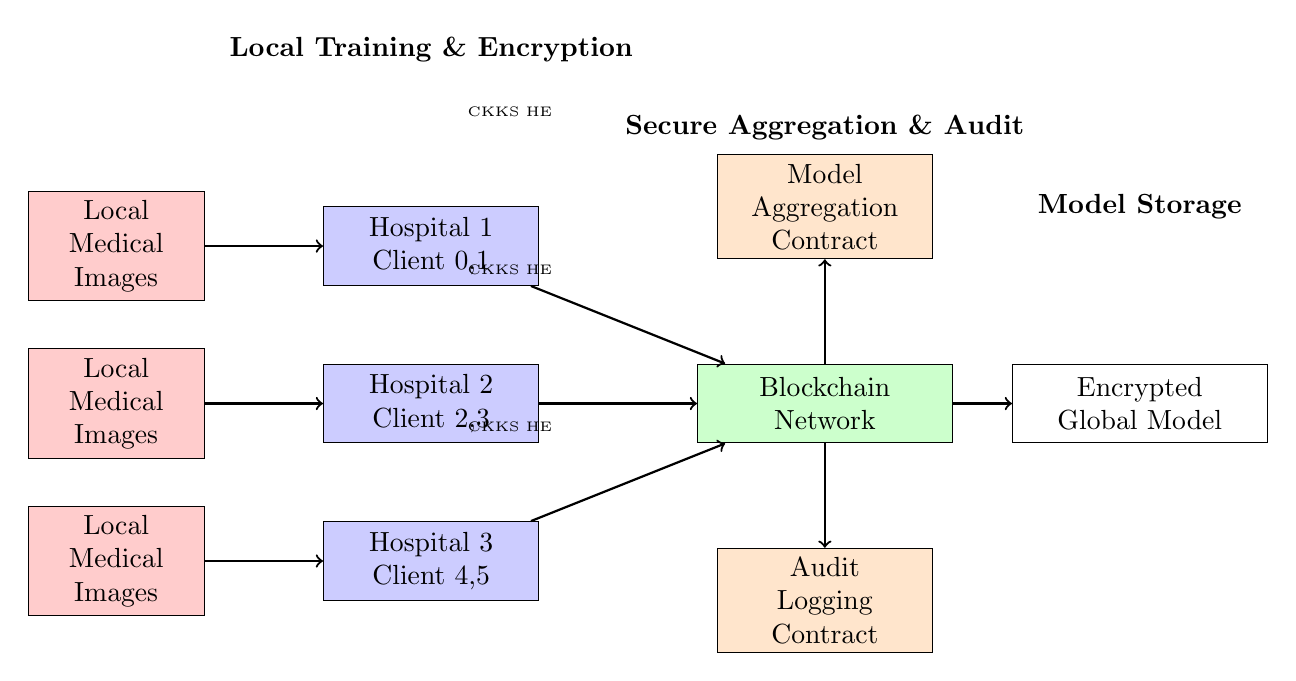
\begin{tikzpicture}[
    node distance=2cm,
    block/.style={rectangle, draw, text width=3cm, text centered, minimum height=1cm},
    client/.style={rectangle, draw, fill=blue!20, text width=2.5cm, text centered, minimum height=1cm},
    blockchain/.style={rectangle, draw, fill=green!20, text width=3cm, text centered, minimum height=1cm},
    contract/.style={rectangle, draw, fill=orange!20, text width=2.5cm, text centered, minimum height=0.8cm},
    arrow/.style={->, thick},
    data/.style={rectangle, draw, fill=red!20, text width=2cm, text centered, minimum height=0.8cm}
]

% Clients
\node[client] (h1) {Hospital 1\\Client 0,1};
\node[client, below of=h1] (h2) {Hospital 2\\Client 2,3};
\node[client, below of=h2] (h3) {Hospital 3\\Client 4,5};

% Local Data
\node[data, left of=h1, xshift=-2cm] (d1) {Local\\Medical\\Images};
\node[data, left of=h2, xshift=-2cm] (d2) {Local\\Medical\\Images};
\node[data, left of=h3, xshift=-2cm] (d3) {Local\\Medical\\Images};

% Blockchain Network
\node[blockchain, right of=h2, xshift=3cm] (bc) {Blockchain\\Network};

% Smart Contracts
\node[contract, above of=bc, yshift=0.5cm] (sc1) {Model\\Aggregation\\Contract};
\node[contract, below of=bc, yshift=-0.5cm] (sc2) {Audit\\Logging\\Contract};

% Global Model
\node[block, right of=bc, xshift=2cm] (gm) {Encrypted\\Global Model};

% Arrows
\draw[arrow] (d1) -- (h1);
\draw[arrow] (d2) -- (h2);
\draw[arrow] (d3) -- (h3);

\draw[arrow] (h1) -- (bc);
\draw[arrow] (h2) -- (bc);
\draw[arrow] (h3) -- (bc);

\draw[arrow] (bc) -- (sc1);
\draw[arrow] (bc) -- (sc2);

\draw[arrow] (bc) -- (gm);

% Labels
\node[above of=h1, yshift=0.5cm] {\textbf{Local Training \& Encryption}};
\node[above of=bc, yshift=1.5cm] {\textbf{Secure Aggregation \& Audit}};
\node[above of=gm, yshift=0.5cm] {\textbf{Model Storage}};

% Encryption labels
\node[above of=h1, xshift=1cm, yshift=-0.3cm] {\tiny CKKS HE};
\node[above of=h2, xshift=1cm, yshift=-0.3cm] {\tiny CKKS HE};
\node[above of=h3, xshift=1cm, yshift=-0.3cm] {\tiny CKKS HE};

\end{tikzpicture}
\end{document} 